\documentclass[15pt]{article}
\usepackage[a4paper, margin=0.85in]{geometry}
\usepackage{amsmath,amsfonts,amsthm} % Math packages
\usepackage[spanish]{babel}
\usepackage{ragged2e}
\usepackage[utf8]{inputenc}
\usepackage{float}
\usepackage[normalem]{ulem}
\useunder{\uline}{\ul}{}
\usepackage{lipsum} % Package to generate dummy text throughout this template
\usepackage{blindtext}
\usepackage{graphicx}
\usepackage{subfigure} % subfiguras
\usepackage{caption}
\usepackage{subcaption}
\usepackage[sc]{mathpazo} % Use the Palatino font
\usepackage[T1]{fontenc} % Use 8-bit encoding that has 256 glyphs
\linespread{1.05} % Line spacing - Palatino needs more space between lines
\usepackage{microtype} % Slightly tweak font spacing for aesthetics
\usepackage{multicol} % Used for the two-column layout of the document
%\usepackage[hang, small,labelfont=bf,up,textfont=it,up]{caption} % Custom captions under/above floats in tables or figures
\usepackage{booktabs} % Horizontal rules in tables
\usepackage{float} % Required for tables and figures in the multi-column environment - they need to be placed in specific locations with the [H] (e.g. \begin{table}[H])
\usepackage{hyperref} % For hyperlinks in the PDF
\usepackage{lettrine} % The lettrine is the first enlarged letter at the beginning of the text
\usepackage{paralist} % Used for the compactitem environment which makes bullet points with less space between them
\usepackage{color}
\sloppy
\definecolor{lightgray}{gray}{0.5}
\setlength{\parindent}{0pt}
\usepackage{abstract} % Allows abstract customization
\renewcommand{\abstractnamefont}{\normalfont\bfseries} % Set the "Abstract" text to bold
\renewcommand{\abstracttextfont}{\normalfont\small\itshape} % Set the abstract itself to small italic text
\usepackage{titlesec} % Allows customization of titles

\renewcommand\thesection{\Roman{section}} % Roman numerals for the sections
%\renewcommand\thesubsection{\Roman{subsection}} % Roman numerals for subsections
\renewcommand{\thesection}{}% Remove section references...
\renewcommand{\thesubsection}{\arabic{subsection}}
\titleformat{\section}[block]{\large\scshape\centering}{\thesection.}{1em}{} % Change the look of the section titles
\titleformat{\subsection}[block]{\large}{\thesubsection.}{1em}{} % Change the look of the section titles
\newcommand{\horrule}[1]{\rule{\linewidth}{#1}} % Create horizontal rule command with 1 argument of height
\usepackage{fancyhdr} % Headers and footers
\pagestyle{fancy} % All pages have headers and footers
\fancyhead{} % Blank out the default header
\fancyfoot{} % Blank out the default footer

\fancyhead[C]{Proyecto final – Econometría II $\bullet$ Universidad de Montevideo $\bullet$ 28 de mayo de 2019} % Custom header text

\fancyfoot[RO,LE]{\thepage} % Custom footer text
%----------------------------------------------------------------------------------------
%       TITLE SECTION
%----------------------------------------------------------------------------------------
\title{\vspace{-10mm}\fontsize{24pt}{12pt}\selectfont\textbf{Research Proposal - Normas de género, ingreso relativo y producción del hogar}} % Article title
\author{
\large
{\textsc{Paula Pereda}}\\[2mm]
}
\date{}

%----------------------------------------------------------------------------------------
\begin{document}
\renewcommand{\figurename}{Figura}
\renewcommand{\tablename}{Tabla}

\maketitle % Insert title
\thispagestyle{fancy} 

\section*{Estrategia de identificación}

Bertrand et al. (2015) encuentran que la distribución de la participación en el ingreso ganado por la esposa exhibe una fuerte caída a la derecha de $\frac{1}{2}$, donde el ingreso de la esposa excede los ingresos del esposo (ver Figura 1). Argumentan que este patrón se explica mejor por las normas de identidad de género, que inducen una aversión a una situación en la que la esposa gana más que su marido.

\begin{figure}[H]
   \caption{Distribution of Relative Income (SIPP Administrative Data)}
   \centering
   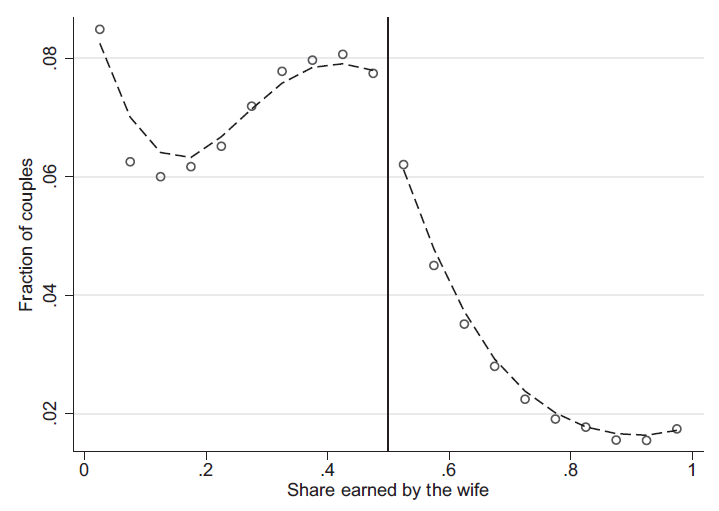
\includegraphics[width=0.7\linewidth]{images/bertrand_2015.png} 
\end{figure}

Utilizando esa discontinuidad como ``norma de género'' (dado que el modelo tradicional de matrimonio no podría explicar tal salto), 
presentan evidencia de que esta aversión también afecta la formación matrimonial, la participación de la fuerza laboral de la esposa, el ingreso de la esposa condicionado al trabajo, la satisfacción matrimonial, la probabilidad de divorcio y la división de la producción doméstica.

\section*{¿Cuál es la pregunta de investigación? ¿Cuál es el efecto causal de interés?}

Mi proyecto consiste primero en encontrar si existe dicha discontinuidad (ver Figuras 2 y 3) y en caso afirmativo, examinar como en el \textit{paper} cómo la violación de la norma de identidad de género (la esposa gana más de la mitad de los ingresos del hogar) afecta la división de la producción doméstica. En el paper, encuentran que la brecha de género en la producción del hogar —dedicación al trabajo no remunerado— es mayor en las parejas donde gana ella más que él. Esto sugiere que una esposa ``amenazadoras'' asume una mayor parte de las tareas domésticas para compensar la violación de la norma.

\newpage

\begin{figure}
\caption{RD Plots – Todos los ingresos, 10 Evenly-Spaced Bins}
\centering
\subfigure[10 Evenly-Spaced Bins (rdrobust)]{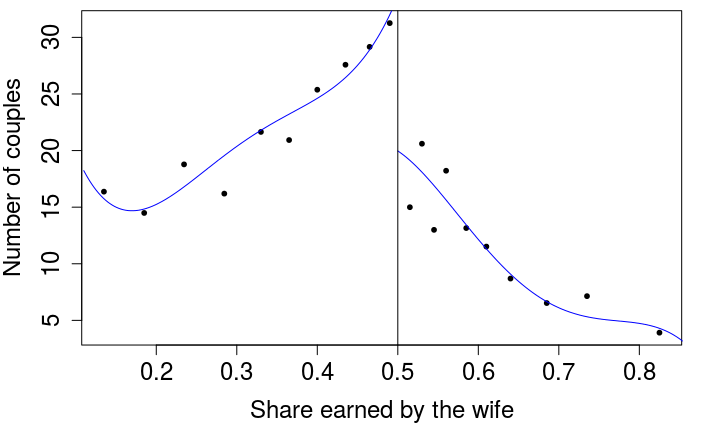
\includegraphics[scale=0.43]{images/rdplot_yt.png}}
\subfigure[10 Evenly-Spaced Bins (rdd)\label{fig:cmos}]{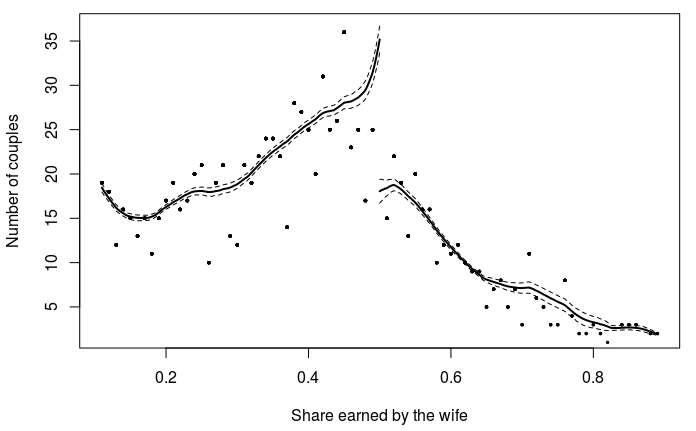
\includegraphics[scale=0.43]{images/rdplot_yt_2.png}}
\end{figure}

\begin{figure}
\caption{RD Plots – Ingresos Laborales, 10 Evenly-Spaced Bins}
\centering
\subfigure[10 Evenly-Spaced Bins (rdrobust)]{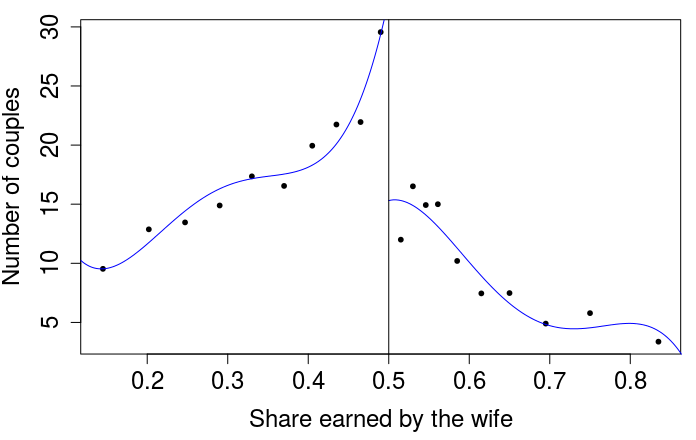
\includegraphics[scale=0.43]{images/rdplot_yl.png}}
\subfigure[10 Evenly-Spaced Bins (rdd)\label{fig:cmos}]{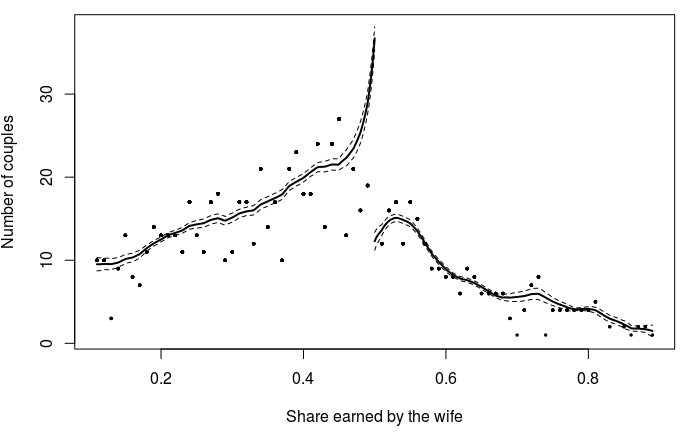
\includegraphics[scale=0.43]{images/rdplot_yl_2.png}}
\end{figure}

\section*{Datos}

Emplearía los datos de la Encuesta Continua de Hogares 2013\footnote{Específicamente la versión criticada y compatibilizada por el IECON para los años 1981-2017.} y la Encuesta de Uso de Tiempo y del Trabajo No Remunerado. Esta última, fue aplicada entre los meses de mayo y agosto de 2013 como módulo extraordinario aplicado revisitando a los hogares relevados por la Encuesta Continua de Hogares (ECH) en marzo de 2013. Se aplicó a 3.391 hogares, obteniéndose información para 7.447 personas de 14 o más años de edad.\\

En esta línea, ambas bases pueden ser ``mergeadas'' por el correlativo y el número de persona en el hogar y me debo quedar con aquellos hogares que efectivamente pueden ser ``mergeados'' y con parejas heterosexuales de 18 a 65 años (3.664 parejas con estas características).\\ 

Todo el código y los datos para reproducir el siguiente documento y los gráficos de RD se encuentran en: \url{https://github.com/paulapereda/proyecto_econometria}

\bibliographystyle{plain}
\bibliography{bib}
\nocite{*}
\end{document}
